\documentclass[tikz,border=12pt]{standalone}
\usepackage{amsmath,amssymb}
\usetikzlibrary{arrows.meta,decorations.pathmorphing,calc}
\definecolor{ink}{HTML}{263145}
\definecolor{accent}{HTML}{4168B3}
\definecolor{warm}{HTML}{B77942}
\tikzset{every picture/.style={font=\small,text=ink},axis/.style={-{Stealth},thin,ink!65},curve/.style={accent,very thick},particle/.style={ink,thick,-{Stealth}}}
\begin{document}

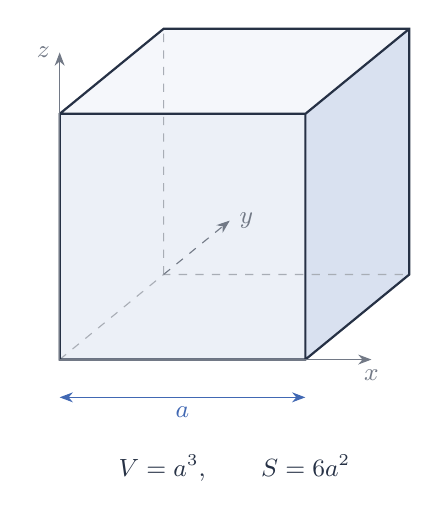
\begin{tikzpicture}[scale=1.2]
\coordinate (O) at (0,0);\coordinate (A) at (2.6,0);\coordinate (B) at (3.7,.9);\coordinate (C) at (1.1,.9);
\coordinate (D) at (0,2.6);\coordinate (E) at (2.6,2.6);\coordinate (F) at (3.7,3.5);\coordinate (G) at (1.1,3.5);
\fill[accent!10] (O)--(A)--(E)--(D)--cycle;
\fill[accent!20] (A)--(B)--(F)--(E)--cycle;
\fill[accent!5] (D)--(E)--(F)--(G)--cycle;
\draw[ink!40,dashed] (O)--(C)--(B) (C)--(G);
\draw[ink,thick] (O)--(A)--(B)--(F)--(G)--(D)--cycle (D)--(E)--(F) (A)--(E);
\draw[axis] (O)--(3.3,0) node[below] {$x$};\draw[axis] (O)--(0,3.25) node[left] {$z$};
\draw[axis,dashed] (C)--(1.8,1.47) node[right] {$y$};
\draw[accent,{Stealth}-{Stealth}] (0,-.4)--(2.6,-.4) node[midway,below] {$a$};
\node at (1.85,-1.15) {$V=a^3,\qquad S=6a^2$};
\end{tikzpicture}
\end{document}
